
\section{Árboles de Merkle}

\subsection{Definición}

Es un \'arbol donde cada nodo contiene el hash de la concatenación de los hashes de sus hijos y las hojas contienen el hash del valor a proteger. En el nodo ra\'iz queda el hash que representa a todo el \'arbol, es decir que si alguno de los nodos modifica su hash invalidar\'a el hash de los nodos padres.

Fue patentado por Ralph Merkle en 1979, como m\'etodo de firmas digitales para robustecer el sistema criptogr\'afico presentado Diffie, Hellman y \'el dos a\~nos antes.

Se lo puede pensar como una estructura de datos más eficiente que las listas enlazadas para la verificación de gran cantidad de datos. 

El árbol de Merkle no requiere ningún algoritmo de hash en particular, siendo posible elegir el más apropiado para cada caso. En general se usa SHA-2.

En la siguiente figura se muestra la estructura de un árbol de Merkle binario, uno de los tipos de árboles más comunes.

\begin{figure}[H]
\centering
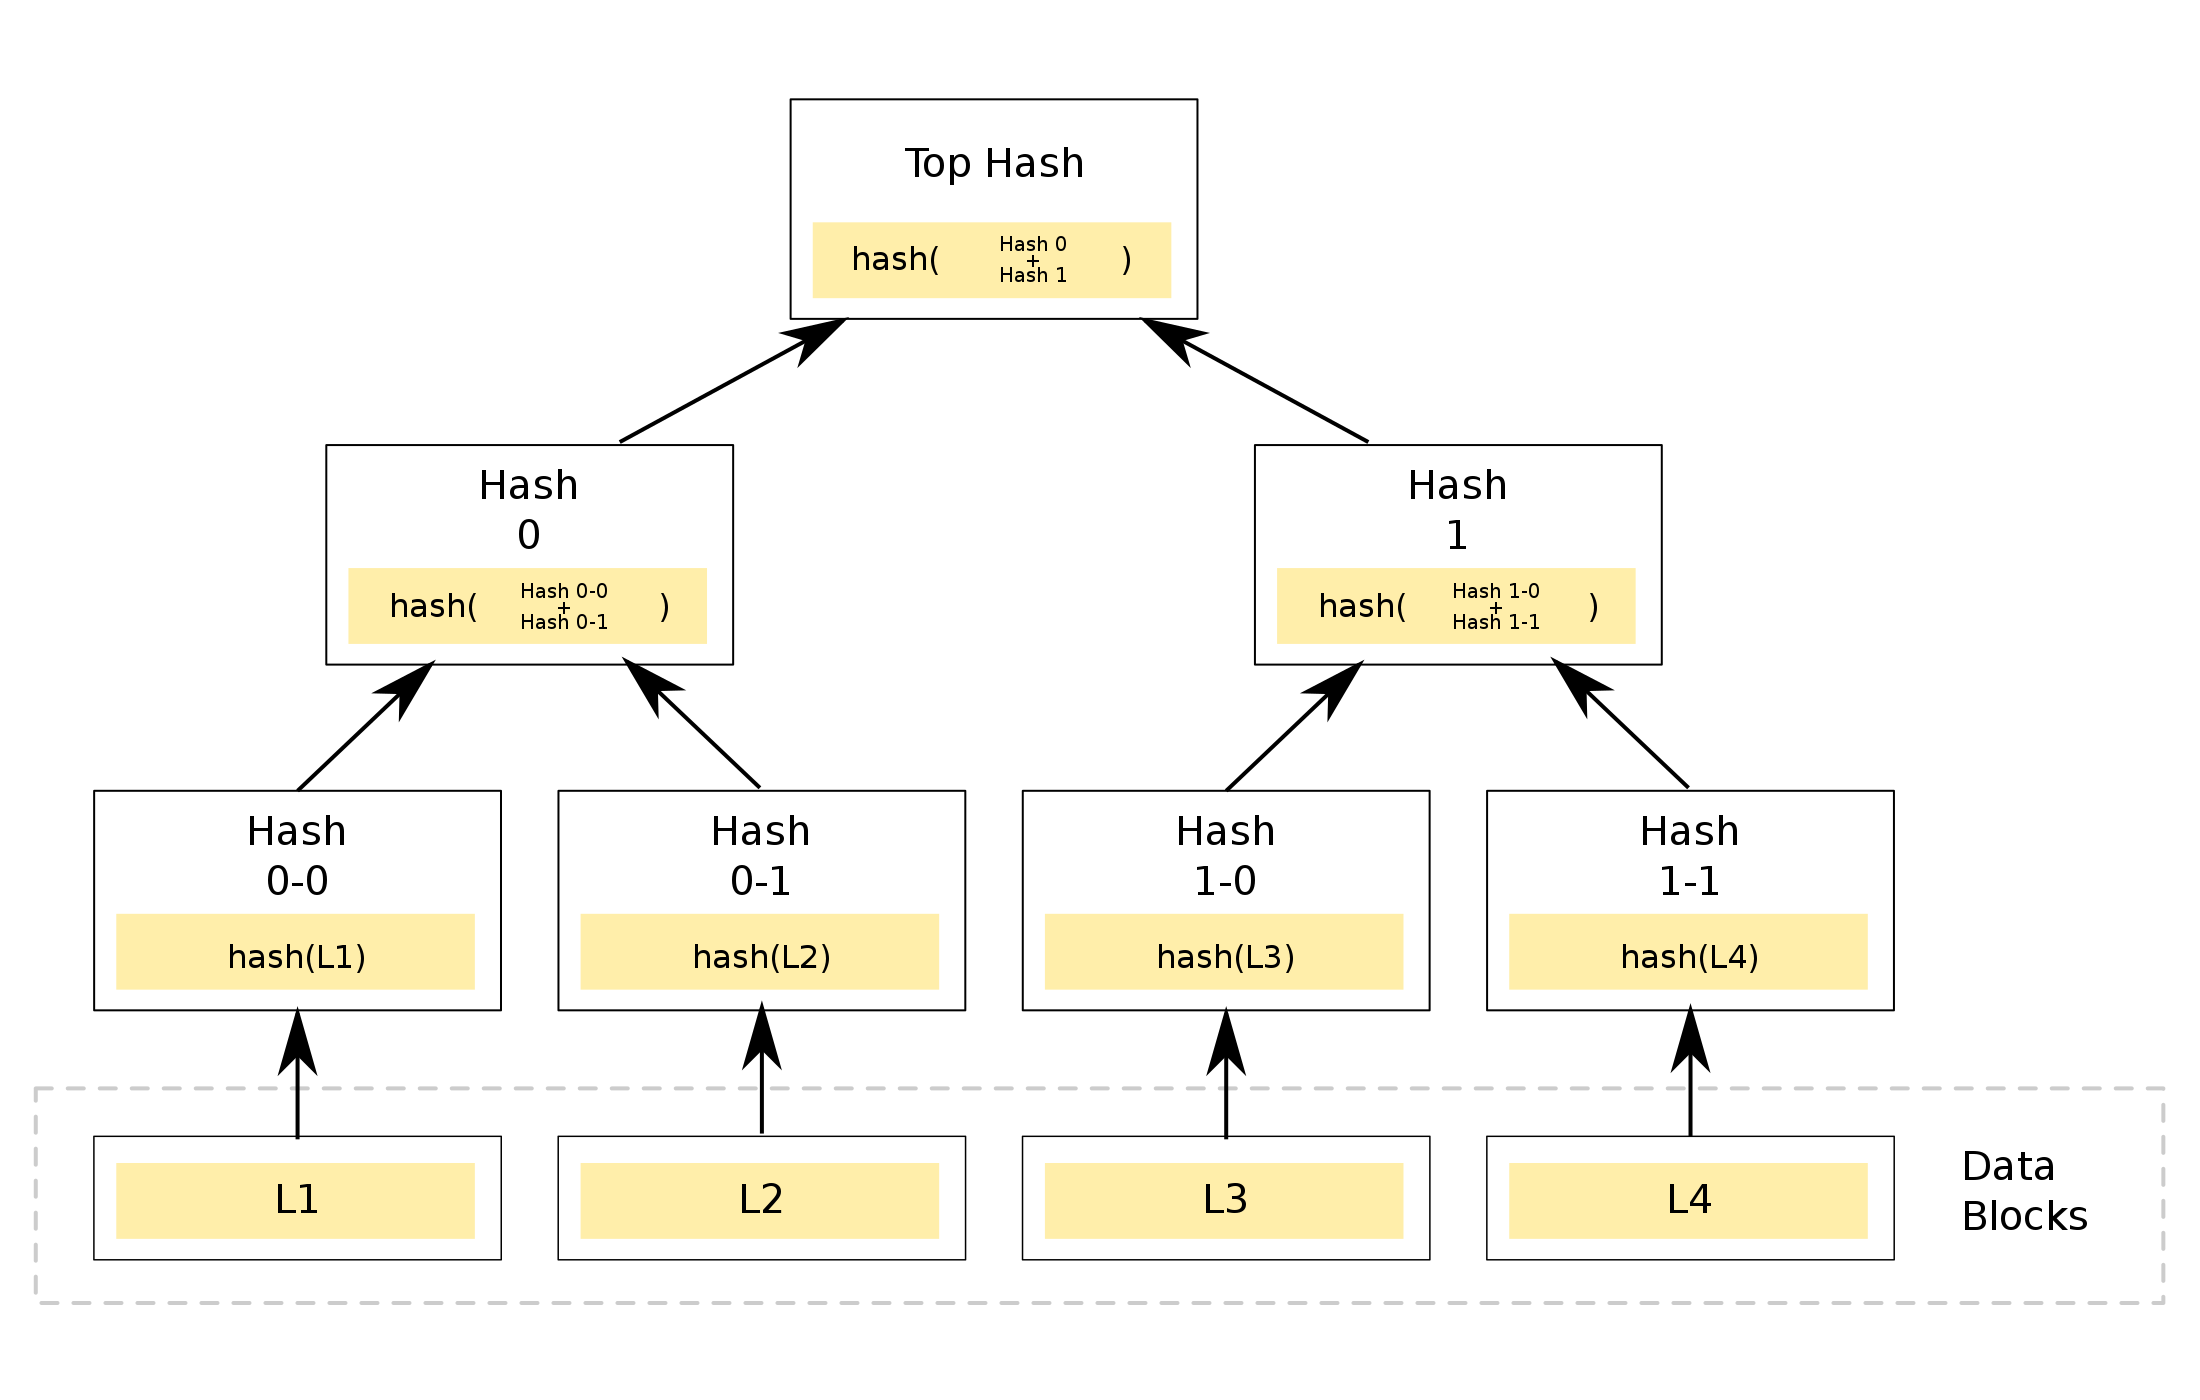
\includegraphics[scale=0.19]{imagenes/hash_tree.png}
\caption{Árbol de Merkle binario}
\end{figure}


\subsection{Principales caracter\'isticas}

\begin{itemize}

\item Merkle Audit Paths: Permite verificar si un bloque de datos protegido fue modificado con \'orden log(n), donde n es la cantidad de bloques de datos totales del \'arbol. As\'i s\'olo requiere calcular 2 * log2(n) hashes, correspondientes al camino desde la ra\'iz al valor a validar junto con los hijos de cada nodo del camino. La misma operaci\'on en listas de hash tiene orden n. Esta es la propiedad más frecuentemente utilizada.

\item Merkle Consistency Proofs: Dada una lista de los primeros m bloques de datos permite verificar no se hayan borrado o agregado algunos, o modificado el \'orden entre ellos. Es una propiedad \'util para mejorar el syslog server ya que además de detectar una modificación en alguna linea de log permite poder seguir verificando las siguientes lineas cosa imposible en la implementación presentada en este trabajo práctico porque el MAC de cada linea depende del anterior.

\end{itemize}


\subsection{Algunos usos}

\subsubsection{Certificate Transparency}
Framework open source para el monitoreo y auditor\'ia de certificados digitales. A partir de un registro p\'ublico de la emisi\'on de los certificados los clientes pueden verificar su validez.

Surgió como necesidad de identificar una gran cantidad de certificados fraudulentos emitidos sin la autorización de las entidades certificantes que supuestamente los habían emitido. El problema se agrava por el tiempo necesario para revocar esos certificados y que los browsers los incluyan en las nuevas versiones.

\begin{figure}[H]
  \centering
  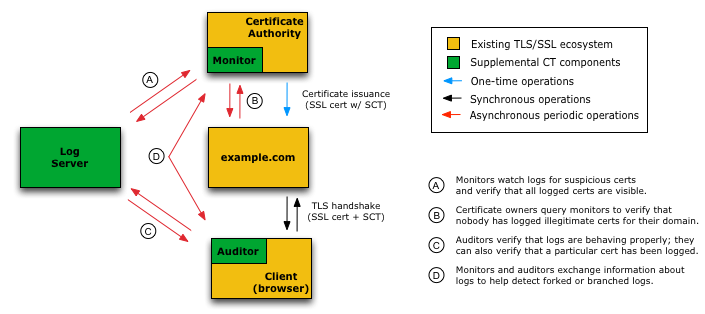
\includegraphics[scale=0.6]{imagenes/ct_system.png}
  \caption{Arquitectura}
\end{figure}

En la figura anterior se pueden observar en verde los componentes de Certificate Transparency agregados al actual ecosistema TCL/SSL. El Log Server es el encargado de mantener el Merkle Tree formado con el registro de la emsión de cada certificado emitido.

\begin{figure}[H]
  \centering
  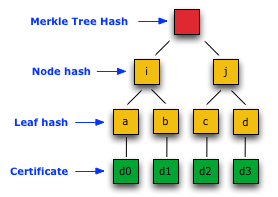
\includegraphics[width=.3\linewidth]{imagenes/ct_hash_1.png}
  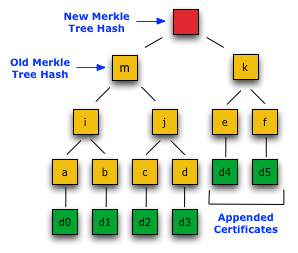
\includegraphics[width=.3\linewidth]{imagenes/ct_hash_2.png}
  \caption{Construcci\'on incremental del \'arbol}
\end{figure}

La figura anterior muestra cómo se agregan más nodos, en este caso registros de emisión de certificados, al árbol de hashes existente, resultando un nuevo árbol que incluye la información intacta del existente. El nuevo árbol tiene un nuevo nodo raíz, con el árbol existente como hijo izquierdo y a la derecha se agregan los nuevos certificados. Este es un ejemplo interesante porque muestra un uso atípico de estos árboles donde no es necesario tener una raíz inmutable para aprovechar sus propiedades de validación.


\subsubsection{Sistemas distribuidos}

En sistemas distribuidos encontramos una gran cantidad de sistemas que hacen uso de estos árboles. Entre ellos hay filesystems como IPFS, sistemas de control de versiones como Git o Mercurial, y bases de datos NoSQL como Cassandra o Dynamo.

Entre los sistemas p2p más populares están BitTorrent, donde el identificador de cada torrent es el root hash del árbol generado a partir de los hashes de las partes del archivo compartido, así esas partes se pueden descargar de cualquier seed siendo sencillo verificar su validez independientemente del resto de las partes.

El sistema distribuido con el mayor poder de cómputo actual, Bitcoin, también lo utiliza. Lo describiremos brevemente para mostrar un ejemplo de árbol estático aportando un beneficio espacial además del temporal. 

\paragraph{Bitcoin}

La red Bitcoin se puede pensar como gran una base de datos distribuida e inmutable donde cada entrada es una transacción generada en la red. Esta base de datos es el blockchain, que como su nombre lo indica, es una cadena de bloques donde cada bloque conoce al anterior y contiene las transacciones realizadas aproximadamente durante los 10 minutos antes de ser agregadal blockchain. 

\begin{figure}[H]
\centering
  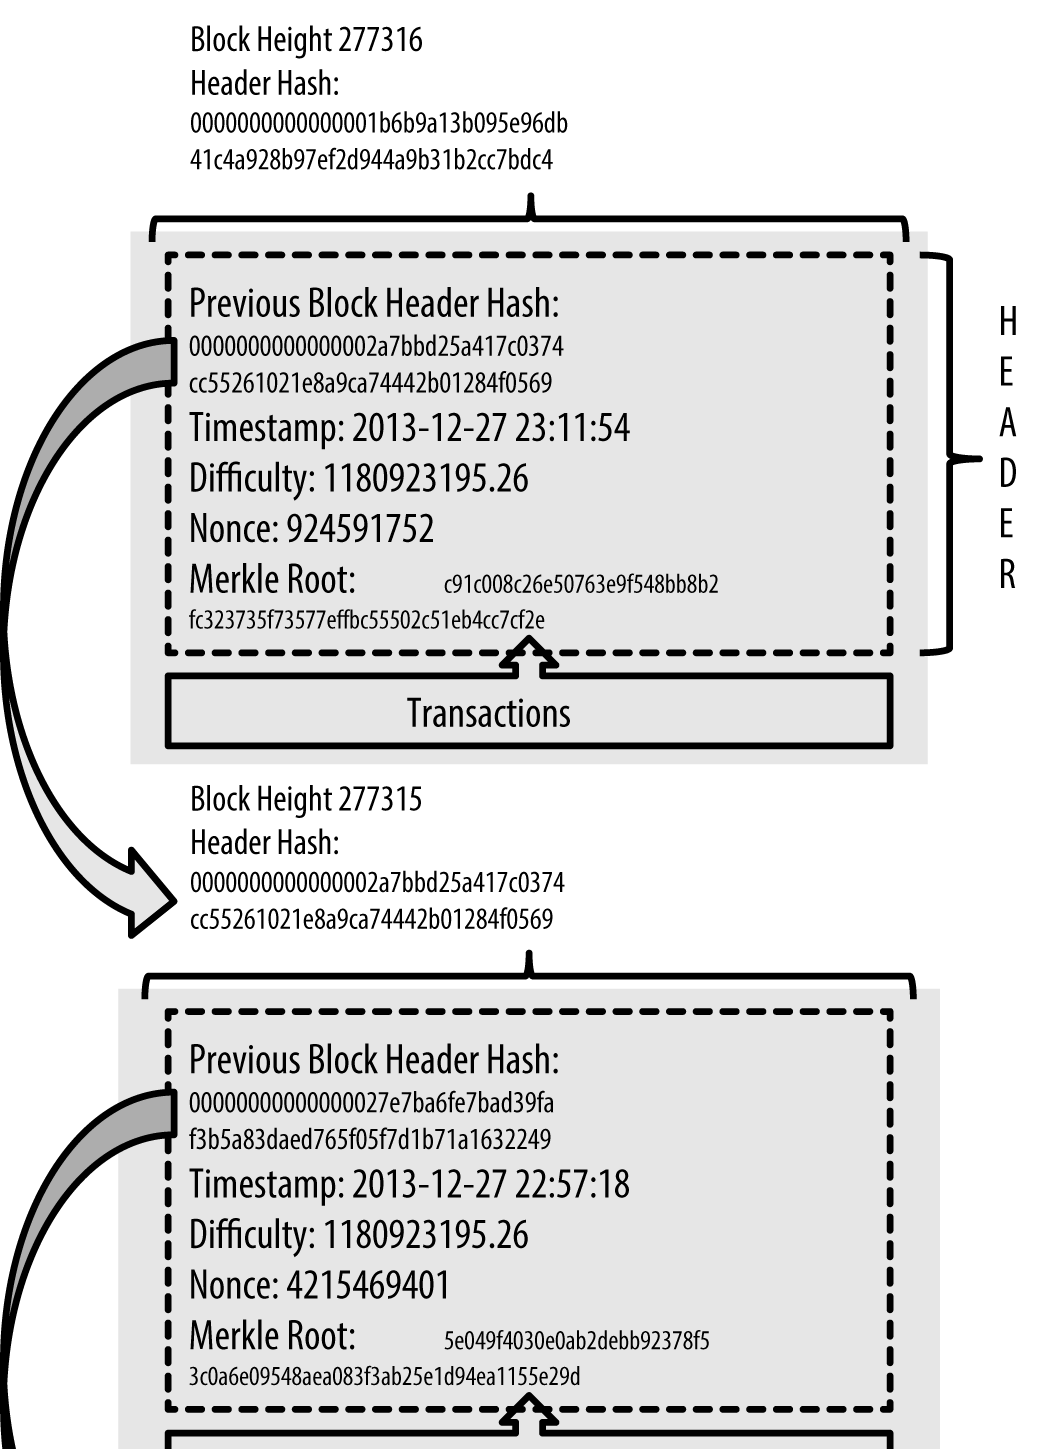
\includegraphics[width=.40\linewidth]{imagenes/blockchain.png}
  \caption{Un par de bloques del blockchain de Bitcoin}
\end{figure}

En el header del bloque de la imagen anterior se puede ver el campo Merkle Root, siendo el nodo raíz del árbol de hashes generado a partir de todas las transacciones de ese bloque. Notar que el header además contiene el hash del bloque anterior y el hash del bloque se calcula sólo sobre el header y no se incluyen las transacciones, alcanza incluir solamente el Merkle Root para validar la integridad de las transacciones.


\begin{figure}[H]
\centering
  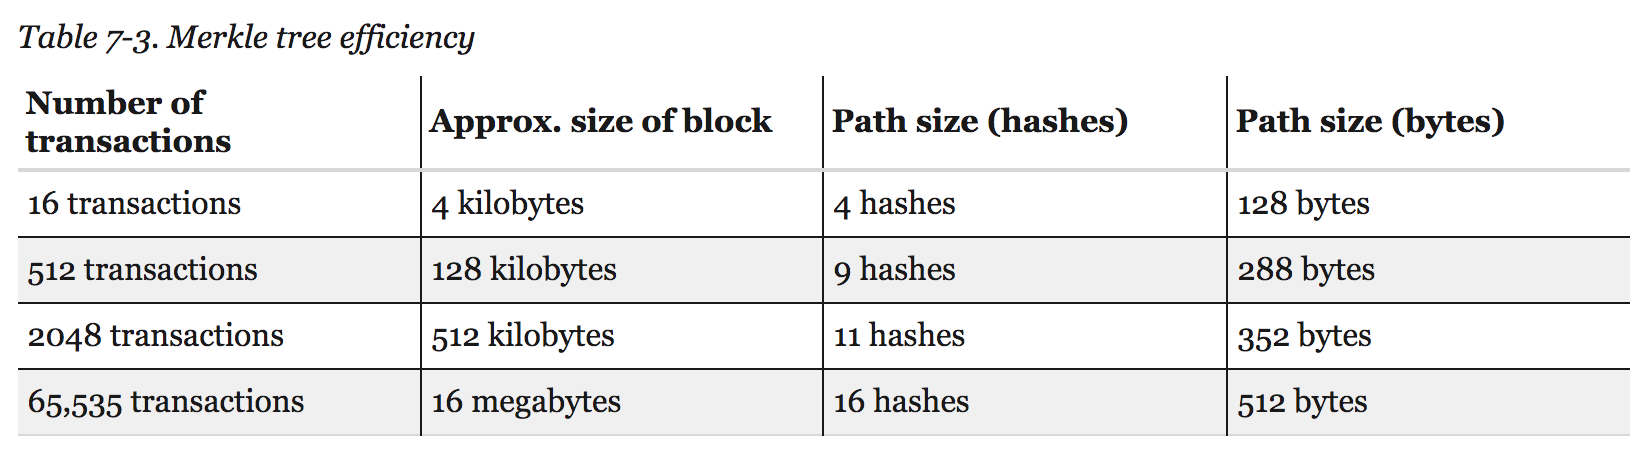
\includegraphics[width=\linewidth]{imagenes/mt_efficiency.png}
\end{figure}

En esta tabla se puede observar la eficiencia del \'arbol de Merkle seg\'un aumenta el camino de Merkle para validar si una transacci\'on es parte de un bloque.

As\'i un nodo puede bajarse s\'olo los bloques de los headers (80 bytes por bloque) para esa validaci\'on y evita bajarse el blockchain completo que puede de varios gigabytes. Estos nodos, usados s\'olo para verificaci\'on de transacciones se llama simplified payment verification (nodos SPV). 







